This simple guide is intended to explain the style used in this documentation.  We request that you follow it as closely as possible when creating content in order to maintain a clear, concise and easy to read body of work.

The documentation was created with and is maintained with \LaTeX.  That stands to reason that much of the formatting is software-dependent, leaving us to worry about more important things.  But that still leaves some decisions for us to make.  For example, alphabetization, certain punctuation, spelling and hyphenation of certain words, and the like will be accounted for here.


\section{alphabetization}

What should and should not be alphabetized:

\begin{itemize}

\item
  General terms such as ``requirements'' or ``specifations'' not used in a ProR or Eclipse specific manner are written in lower-case.
\item
  ProR- and Eclipse-specific terms shall be capitalized. i.e., terms such as ``Eclipse Workbench,'' ``SpecObject,'' ``Editor,'' and ``Views'' are capitalized.

\end{itemize}

\section{Punctuation}

\begin{itemize}

\item
  \textbf{Mdashes} shall be used when needed—here is a perfect example—with no spaces. 
\item
  \textbf{Periods} will be followed by double-spaces.
\item
  When \textbf{Colons} are used to introduce a series of numbered items in a list, do not capitalize the first item after the colon (unless it's a proper noun) and seperate the list items with semi-colons, e.g.:
  There are three differences: (1) the first difference; (2) the second difference; and (3) the third difference.
  
\end{itemize}

**********


\section{Contributing}

Documentation is one of those things that gets easily neglected in open source projects.  It is also one of the easiest for outsiders to contribute to.  The documentation is managed as Latex, which may scare some people.  But no worries, those who don't want to learn Latex don't have to.

There are broadly two ways for contributing to the documentation:

\begin{description}
  \item[File a bug.]  Visit the \href{https://bugs.eclipse.org/bugs/enter_bug.cgi?assigned_to=&blocked=&bug_severity=normal&bug_status=NEW&comment=&contenttypeentry=&contenttypemethod=autodetect&data=&dependson=&description=&flag_type-1=X&flag_type-11=X&flag_type-12=X&flag_type-2=X&flag_type-4=X&flag_type-6=X&flag_type-7=X&flag_type-8=X&form_name=enter_bug&keywords=&&op_sys=All&product=MDT.RMF&qa_contact=&rep_platform=All&short_desc=&version=unspecified}{RMF Bug Tracker}.  You can just point out a problem or request for improvement.  You can also provide some text to be added to the documentation (unformatted).  If you do, however, then you need to sign a Committer License Agreement (CLA)
  \item[Submit improved \LaTeX via Gerrit.]  If you are technically inclined (meaning that you know what \LaTeX and git are, and how to use them), then you can contribute via the Gerrit code review system, as described \href{https://wiki.eclipse.org/Gerrit}{at eclipse.org}.
\end{description}

\subsection{Gerrit for Contributions}

TODO - when done, update the parent section as well.

\section{Licensed as EPL}

This work is licensed under the Eclipse Public License.

\section{Acknowledgements}

Many parties were involved in the creation of RMF.  We would like to thank the core team that made it possible.

\begin{figure}[H]
  \centering
  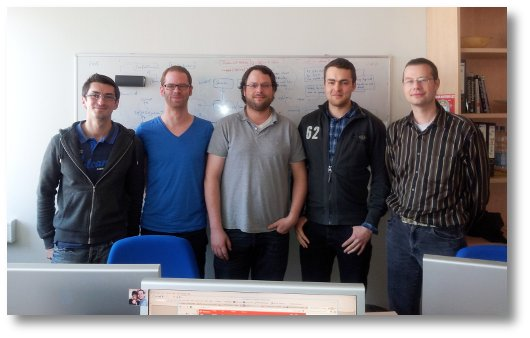
\includegraphics[width=\textwidth]{../rmf-images/2012_03_sprint_team.jpg}
  \caption{The RMF team during a Sprint in April 2012 in Düsseldorf, Germany
  (left to right) Lukas Ladenberger, Mark Brörkens, Ingo Weigelt, Said Salem, Michael Jastram}
  \label{fig:intro_core_team}
\end{figure}


The roots of this project were created by Andreas Graf, Michael Jastram and Nirmal Sasidharan, who joined together individual projects to create RMF.  Their efforts were financed by the research projects itea Verde and FP7 Deploy.  RMF was assembled at the Eclipse Foundation, where it has been active ever since.  Figure~\ref{fig:intro_core_team} shows four of the five RMF Committers at a joint coding session (missing is Andreas Graf).
